% ============================================================
%  CASE STUDY REPORT: Hospital Record Indexing System
%  Course: Advanced Data Structures and Applications (ADSA)
% ============================================================
\documentclass[11pt,a4paper]{article}

\usepackage[T1]{fontenc}
\usepackage[utf8]{inputenc}
\usepackage{lmodern}
\usepackage[margin=1.8cm]{geometry}
\usepackage{amsmath,amssymb}
\usepackage{graphicx}
\usepackage{tikz}
\usetikzlibrary{positioning,arrows.meta,calc}
\usepackage{pgfplots}
\pgfplotsset{compat=1.18}
\usepackage{booktabs}
\usepackage{tabularx}
\usepackage{enumitem}
\usepackage{listings}
\usepackage{titlesec}
\usepackage{float}

% === CLEAN WORD-LIKE FORMATTING ===
\titleformat{\section}{\large\bfseries}{\thesection.}{0.5em}{}
\titlespacing*{\section}{0pt}{10pt}{5pt}
\titleformat{\subsection}{\normalsize\bfseries}{\thesubsection}{0.5em}{}
\titlespacing*{\subsection}{0pt}{8pt}{3pt}

\lstset{
  basicstyle=\small\ttfamily,
  keywordstyle=\bfseries,
  frame=none,
  breaklines=true,
  language=Java,
  showstringspaces=false,
}

\begin{document}

% ==========================================
% 1. TITLE
% ==========================================
\begin{center}
    \includegraphics[width=3cm]{images/pict.jpeg}\\[0.5cm]
    {\Large\bfseries SCTR's Pune Institute of Computer Technology}\\[0.2cm]
    {\large\bfseries CASE STUDY REPORT}\\[1.0cm]
\end{center}

\begin{flushleft}
    \textbf{Title of the Case Study:} Hospital Record Indexing System (Disk-Optimized)\\
    \textbf{Course Name:} Advanced Data Structures and Applications (ADSA)\\
    \textbf{Faculty Name:} [Faculty Name]\\
    \textbf{Group Members:} \\
    1. [Name 1] --- [Roll No.]\\
    2. [Name 2] --- [Roll No.]\\
    3. [Name 3] --- [Roll No.]\\
    4. [Name 4] --- [Roll No.]\\[0.3cm]
    \textbf{Date of Submission:} [Date]
\end{flushleft}

\hr
% ==========================================
% 2. PROBLEM STATEMENT
% ==========================================
\section{Problem Statement}
A hospital requires a system to manage millions of patient records stored on disk. The system must support:
\begin{itemize}[noitemsep]
    \item Fast exact search for a Patient ID.
    \item Efficient range queries (retrieving IDs in a specific interval).
    \item Frequent insertions as new patients arrive.
    \item \textbf{Minimal disk I/O}, as fetching from disk is extremely slow compared to memory.
\end{itemize}
The key challenge is providing $O(\log n)$ performance while minimizing the number of disk blocks read.

% ==========================================
% 3. PROBLEM ANALYSIS
% ==========================================
\section{Problem Analysis}
\textbf{System Requirements:}
\begin{itemize}[noitemsep]
    \item Data is too large for RAM; it must reside on secondary storage.
    \item High fan-out required to keep tree height low.
\end{itemize}
\textbf{Operations:}
\begin{itemize}[noitemsep]
    \item \texttt{search(id)}: Locate a specific record.
    \item \texttt{insert(record)}: Add a new patient.
    \item \texttt{rangeQuery(low, high)}: Retrieve continuous records.
\end{itemize}
\textbf{Constraints:} Disk latency is high. Each operation should involve minimum node transitions.

% ==========================================
% 4. DATA STRUCTURE SELECTION \& JUSTIFICATION
% ==========================================
\section{Data Structure Selection \& Justification}
\begin{table}[H]
\small
\begin{tabularx}{\textwidth}{@{}l l X@{}}
\toprule
\textbf{Operation} & \textbf{Data Structure} & \textbf{Justification}\\
\midrule
Exact Search & B-Tree & Multi-way branching minimizes tree height, reducing disk reads.\\
Range Query & B-Tree & Keys are stored in sorted order; sequential access is efficient.\\
Insertion & B-Tree & Self-balancing ensures consistent $O(\log n)$ performance.\\
Disk Storage & B-Tree & Node size can be aligned with disk block size (e.g., 4KB).\\
\bottomrule
\end{tabularx}
\end{table}

% ==========================================
% 5. SYSTEM ARCHITECTURE
% ==========================================
\section{System Architecture}
\begin{center}
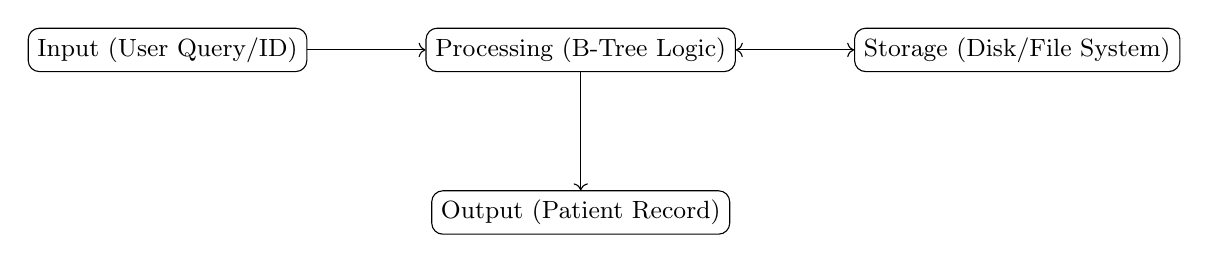
\begin{tikzpicture}[node distance=1.5cm, every node/.style={draw, rounded corners, align=center, font=\small}]
    \node (in) {Input (User Query/ID)};
    \node (proc) [right=of in] {Processing (B-Tree Logic)};
    \node (store) [right=of proc] {Storage (Disk/File System)};
    \node (out) [below=of proc] {Output (Patient Record)};
    
    \draw[->] (in) -- (proc);
    \draw[->] (proc) -- (store);
    \draw[<-] (proc) -- (store);
    \draw[->] (proc) -- (out);
\end{tikzpicture}
\end{center}

\newpage
% ==========================================
% 6. WORKFLOW / ALGORITHM DESIGN
% ==========================================
\section{Workflow / Algorithm Design}
The system follows a top-down traversal for all operations.

\begin{lstlisting}
// Java-style Pseudocode for Search
void search(Node x, int key) {
    int i = 0;
    while (i < x.count && key > x.id_list[i]) i++;
    if (i < x.count && key == x.id_list[i]) {
        print(x.data_list[i]);
        return;
    }
    if (x.leaf) return; 
    search(x.children[i], key); 
}
\end{lstlisting}

% ==========================================
% 7. DATA FLOW DIAGRAM (DFD)
% ==========================================
\section{Data Flow Diagram (DFD)}
\begin{center}
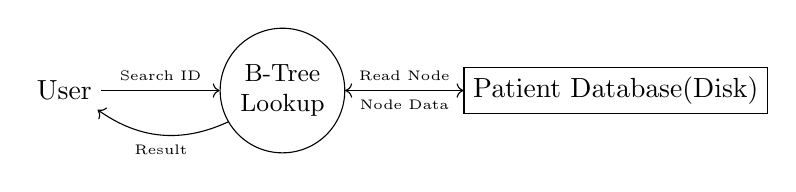
\begin{tikzpicture}[node distance=1.5cm, circle_node/.style={draw, circle, align=center, font=\small}]
    \node[draw=none] (user) {User};
    \node[circle_node, right=of user] (p1) {B-Tree\\Lookup};
    \node[draw, rectangle, right=of p1] (db) {Patient Database\\(Disk)};
    
    \draw[->] (user) -- node[above, font=\tiny] {Search ID} (p1);
    \draw[->] (p1) -- node[above, font=\tiny] {Read Node} (db);
    \draw[<-] (p1) -- node[below, font=\tiny] {Node Data} (db);
    \draw[->] (p1) to [bend left] node[below, font=\tiny] {Result} (user);
\end{tikzpicture}
\end{center}

% ==========================================
% 8. SAMPLE INPUT \& OUTPUT
% ==========================================
\section{Sample Input \& Output}
\textbf{Input:}
\begin{itemize}[noitemsep]
    \item Insertion: ID=102, Name="John Doe"
    \item Search: ID=102
\end{itemize}
\textbf{Output:}
\begin{itemize}[noitemsep]
    \item "Patient Record Added Successfully."
    \item "Found: ID: 102 | Name: John Doe | History: Fever | Billing: 500"
\end{itemize}

% ==========================================
% 9. COMPLEXITY ANALYSIS
% ==========================================
\section{Complexity Analysis}
\begin{itemize}[noitemsep]
    \item \textbf{Time Complexity:} $O(\log_m n)$, where $m$ is the tree order. With branching factor of 100, a tree with 1 million records has a height of only $\approx 3$.
    \item \textbf{Space Complexity:} $O(n)$ to store keys and pointers on disk.
\end{itemize}

% ==========================================
% 10. COMPARISON WITH ALTERNATIVE APPROACH
% ==========================================
\section{Comparison with Alternative Approach}
\begin{itemize}[noitemsep]
    \item \textbf{AVL/Red-Black Tree:} These are memory-optimized. In disk storage, each node is a separate disk read. A tree for 1 million records would have a height of $\approx 20$, requiring 20 disk seeks.
    \item \textbf{B-Tree:} Requires only $\approx 3$ disk seeks for the same data size.
\end{itemize}

% ==========================================
% 11. APPLICATIONS \& BENEFITS
% ==========================================
\section{Applications \& Benefits}
\begin{itemize}[noitemsep]
    \item Databases (SQL/NoSQL) and File Systems (NTFS, HFS+).
    \item Benefits: Highly scalable, stable performance, and native support for range queries.
\end{itemize}

% ==========================================
% 12. CONCLUSION
% ==========================================
\section{Conclusion}
The B-Tree is an ideal choice for hospital indexing due to its high fan-out and disk-block alignment. We learned how tree depth impacts I/O performance and how multi-way trees solve large-scale data storage problems.

\end{document}